\subsection{Software-Architektur}
	\subsubsection{Systemübersicht}
	Zur Übersicht über den erarbeiteten Lösungsansatz bietet sich die Darstellung durch ein Kontextdiagramm an. Darin zu erkennen sind die fünf Hauptkomponenten  DesktopViewer, CoreApp, Detector, MediaCommunication und ControllerCommunication. Weiter enthält das System mindestens drei Schnittstellen, einerseits die Bluetooth Schnittstelle zwischen Startgerät und Ballwerfer, des Weiteren die muss die Kommunikation mit Kamera und Controller gewährleistet sein. Die Schnittstelle zur Kamera sollte, sofern wie geplant ein Smartphone verwendet wird, bereits durch das entsprechende Betriebssystem gegeben sein, weshalb in diesem Dokument nicht weiter auf diese Schnittstelle eingegangen wird.
  fehlt noch
\begin{figure}[h!]
		\centering
		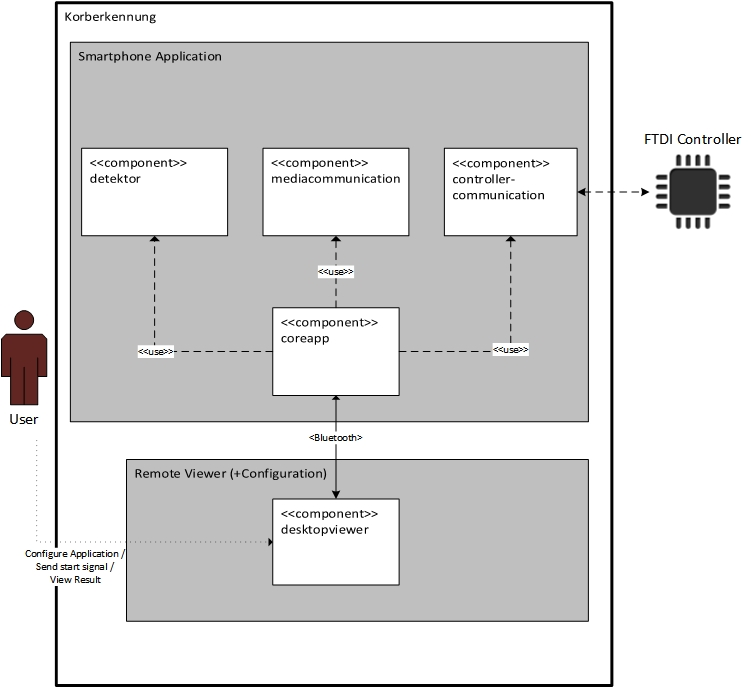
\includegraphics[width=0.9\textwidth]{Enddokumentation/Loesungskonzept/Bilder/Kontextdiagramm_v2.jpg}
		\caption{Kontextdiagramm}		
\end{figure}


	\subsubsection{Komponenten-Spezifikation}
		\paragraph{DesktopViewer\\}
		Über die Viewer-Komponente wird die Konfiguration der Applikation, sowie die Auslösung des Startsignals realisiert. Weiter soll es zu Testzwecken möglich sein, die Resultate der Korberkennung ebenfalls über den DesktopViewer zu betrachten.
		
		\paragraph{CoreApp\\}
		Als Kernbestandteil der Smartphone App umfasst die CoreApp-Komponente auf der einen Seite die Kommunikation mit der Viewer-Komponente, auf der anderen Seite wird hier der Ablauf der Kernfunktionen zur Objekterkennung koordiniert.
		
		\paragraph{Detector\\}
		Dem Detektor muss ein Bild übergeben werden, welches von diesem darauf ausgewertet wird. Dabei sucht der Detektor nach einem dunkeln Objekt im Bild und ist in der Lage, anhand der ermittelten Position den Winkel des Ballwerfers zum Korb bestimmen kann.
		
		\paragraph{MediaCommunication\\}
		In dieser Komponente ist die Kommunikation mit der Kamera des Smartphones umgesetzt. Hauptsächlich geht es darum, ein Foto aufzunehmen, welches wiederrum dem Detektor zur Winkelbestimmung übergeben wird.
		
		\paragraph{ControllerCommunication\\}
		Wie der Name bereits sagt wird an dieser Stelle die Kommunikation mit dem FTDI-Controller realisiert. Der vom Detektor berechnete Winkel wird hier übertragen um anschliessend Mechanisch umgesetzt zu werden und den Ballwerfer aufs Ziel auszurichten.
		
	\subsubsection{Schnittstellen-Spezifikation}
		% Übersicht Schnittstellen fehlt Schnittstellen
		\begin{figure}[h!]
			\centering
			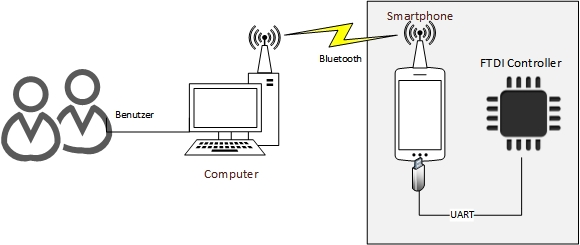
\includegraphics[width=0.9\textwidth]{Enddokumentation/Loesungskonzept/Bilder/Schnittstellen.jpg}
			\caption{Schnittstellen}		
		\end{figure}
		Als weiteres Hauptelement des entworfenen Systems werden im nachfolgenden Abschnitt die in der Grafik erkennbaren Schnittstellen (Bluetooth und Controller) deklariert.
		
		\paragraph{Bluetooth\\}
		Die Kommunikation vom Startgerät (Notebook) zum Smartphone (Android Device auf dem Ballwerfer) für die Übermittlung des Startsignals findet mit Bluetooth statt. Die Bluetooth-Komponente auf dem Notebook startet nach Aktivierung ein ‚inquiry‘ (Erkundigung) nach verfügbaren Bluetooth-Geräten. Anschliessend wird eine Service-Anfrage (RFCOMM, eine COM-Schnittstelle) an ein gewünschtes Bluetooth-Gerät gestartet, bei positiver Rückmeldung werden die zwei Geräte gepaart. Eine uni- oder bidirektionale Kommunikation zwischen den Geräten kann nun jederzeit aufgebaut werden. Das eigentliche Startsignal wird ein primitiver Datentyp sein.
		
		\paragraph{Controller\\}
		Die Verbindung vom Android Smartphone zum FTDI Controller wird mit USB realisiert. 
		Das Smartphone kommuniziert über den bereitgestellten Treiber von FTDI mit dem Controller, die verwendete Schnittstelle ist UART. Die Kommunikation ist soll bidirektional sein, kann also sowohl empfangen als auch senden. Der Vorteil einer solchen Verbindung ist das sie als COM-Schnittstelle angesteuert werden kann was relativ einfach zu implementieren ist. Die Verbindung ist ausfallsicher und einfach aufrechtzuerhalten.		
		
	\subsubsection{Funktionale Sicht}
	
	\begin{figure}[h!]
		\centering
		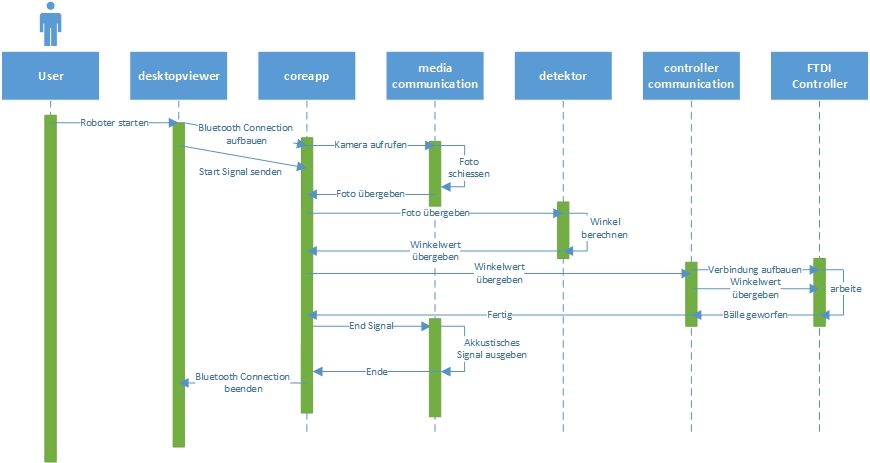
\includegraphics[width=0.9\textwidth]{Enddokumentation/Loesungskonzept/Bilder/Sequenzdiagramm.jpg}
		\caption{Sequenzidagramm}		
	\end{figure}
Ein User gibt den Startbefehl für den Roboter durch die Komponente desktopviewer, die auf einem Computer ausgeführt wird. Desktopviewer baut eine Bluetooth-Connection mit der Komponente Coreapp, welche auf dem Smartphone ausgeführt wird, und sendet anschliessend das Startsignal welches durch den User aufgerufen wird. \\
Ab diesem Zeitpunkt läuft die Applikation völlig autonom. Die coreapp ruft als erstes die mediacommunication Komponente auf und schiesst ein Foto. Das Foto wird an die coreapp zurückgegeben.
Die Komponente coreapp ruft die Komponente 	detektor auf und übergibt dieser das Foto, welche daraufhin den Winkel ausrechnet und diesen an coreapp übergibt.\\
Der berechnete Winkel wird an die Komponente controllercommunication übergeben. Die Komponente baut die Verbindung zum FTDI-Controller auf und übergibt diesem den Winkelwert, danach wartet die Komponente bis der FTDI-Controller das Ende des Ballwurfes zurückgibt. Controllercommuncation übergibt an die Coreapp die Meldung das der Roboter fertig ist. \\
Coreapp ruft die medacommunication Komponente auf welche das Programmende signalisiert.
		
		
